% File generated by nTex - Java Application for fast notes in LaTeX
% by Jarda Vitku

\documentclass[journal,onecolumn]{IEEEtrancz}
% zvolte kodovani
\usepackage[utf8]{inputenc} % linux/unix
%\usepackage[latin2]{inputenc}
%\usepackage[cp1250]{inputenc} % Windows
\usepackage[czech]{babel}
\usepackage{graphicx}
\usepackage{makeidx}         % allows index generation
\usepackage[bookmarks=false, colorlinks=false, unicode]{hyperref}

%\usepackage{enumitem}
%\setlistdepth{9}

\begin{document}

\title{ doc }
\author{Jaroslav Vítků}

\maketitle

\begin{abstract}
	abs 
\end{abstract}

\IEEEpeerreviewmaketitle



%%%%%%%%%%%%%%%%%%%%%%%%%%%%%% text

\section{sec}
text..

\subsection{sub}
citation \cite{kniha}, figure: Obr.\ref{a}, reference: Obr.\ref{a} 

\begin{figure}[ht]
	\centering
		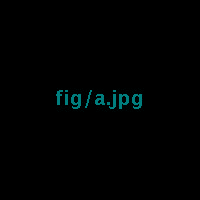
\includegraphics[width=4.0cm]{fig/a.jpg}
	\caption{label}
	\label{a}
\end{figure}





%%%%%%%%%%%%%%%%%%%%%%%%%%%%%% literature
\begin{literatura}{1}

\bibitem{kniha} 
Allman J.: \emph{Evolving Brains}, Scientific American Library Paperback, 2000.
\end{literatura}

\end{document}
